\chapter{考察}\label{cha:Discussion}
本研究では、レイアウトを変更せず、電子フォーム作成にかかる手間と時間を削減することを目的として、記入欄検出およびラベル付与ツールの試作を行った。
試作したツールは、以下に示す2つの機能を持つ。

\begin{itemize}
  \item 領域座標取得およびラベル付与機能
  \item 領域強調画像出力機能
\end{itemize}

本章では、評価実験を行い、試作したツールの有用性を評価する。
また、試作したツールと関連ツールを比較する。
最後に、試作したツールの問題点について述べる。

\section{試作したツールの有用性に関する評価}\label{sec:evalue_usefulness}
試作したツールの有用性を評価するため、試作したツールを、電子フォーム作成ツールであるPhotolize\cite{Photolize}に適用し、実験を行う。
Photolizeは、スマートフォンで撮影した帳票の画像に対して、電子フォーム記入欄をGUIツールで配置することによって、電子フォームの作成を支援するサービスである。
試作したツールをPhotolizeに適用することで、領域座標とラベルをまとめたJSONファイルを参照し、電子フォーム記入欄を自動で配置することによって、電子フォーム記入欄の配置にかかる手間と時間を削減することができる。

実験の対象とした帳票の画像を、図\ref{fig:experiment_A}と図\ref{fig:experiment_B}に示す。
図\ref{fig:experiment_A}は、電子文書の画像であり、図\ref{fig:experiment_B}は、電子化文書の画像である。
以降、図\ref{fig:experiment_A}の画像を、帳票画像A、図\ref{fig:experiment_B}の画像を、帳票画像Bと呼ぶ。
なお、帳票画像記入欄の数は、それぞれ図\ref{fig:experiment_A}が54個、図\ref{fig:experiment_B}が48個である。

\begin{figure}[t]
    \begin{center}
        \fbox{
            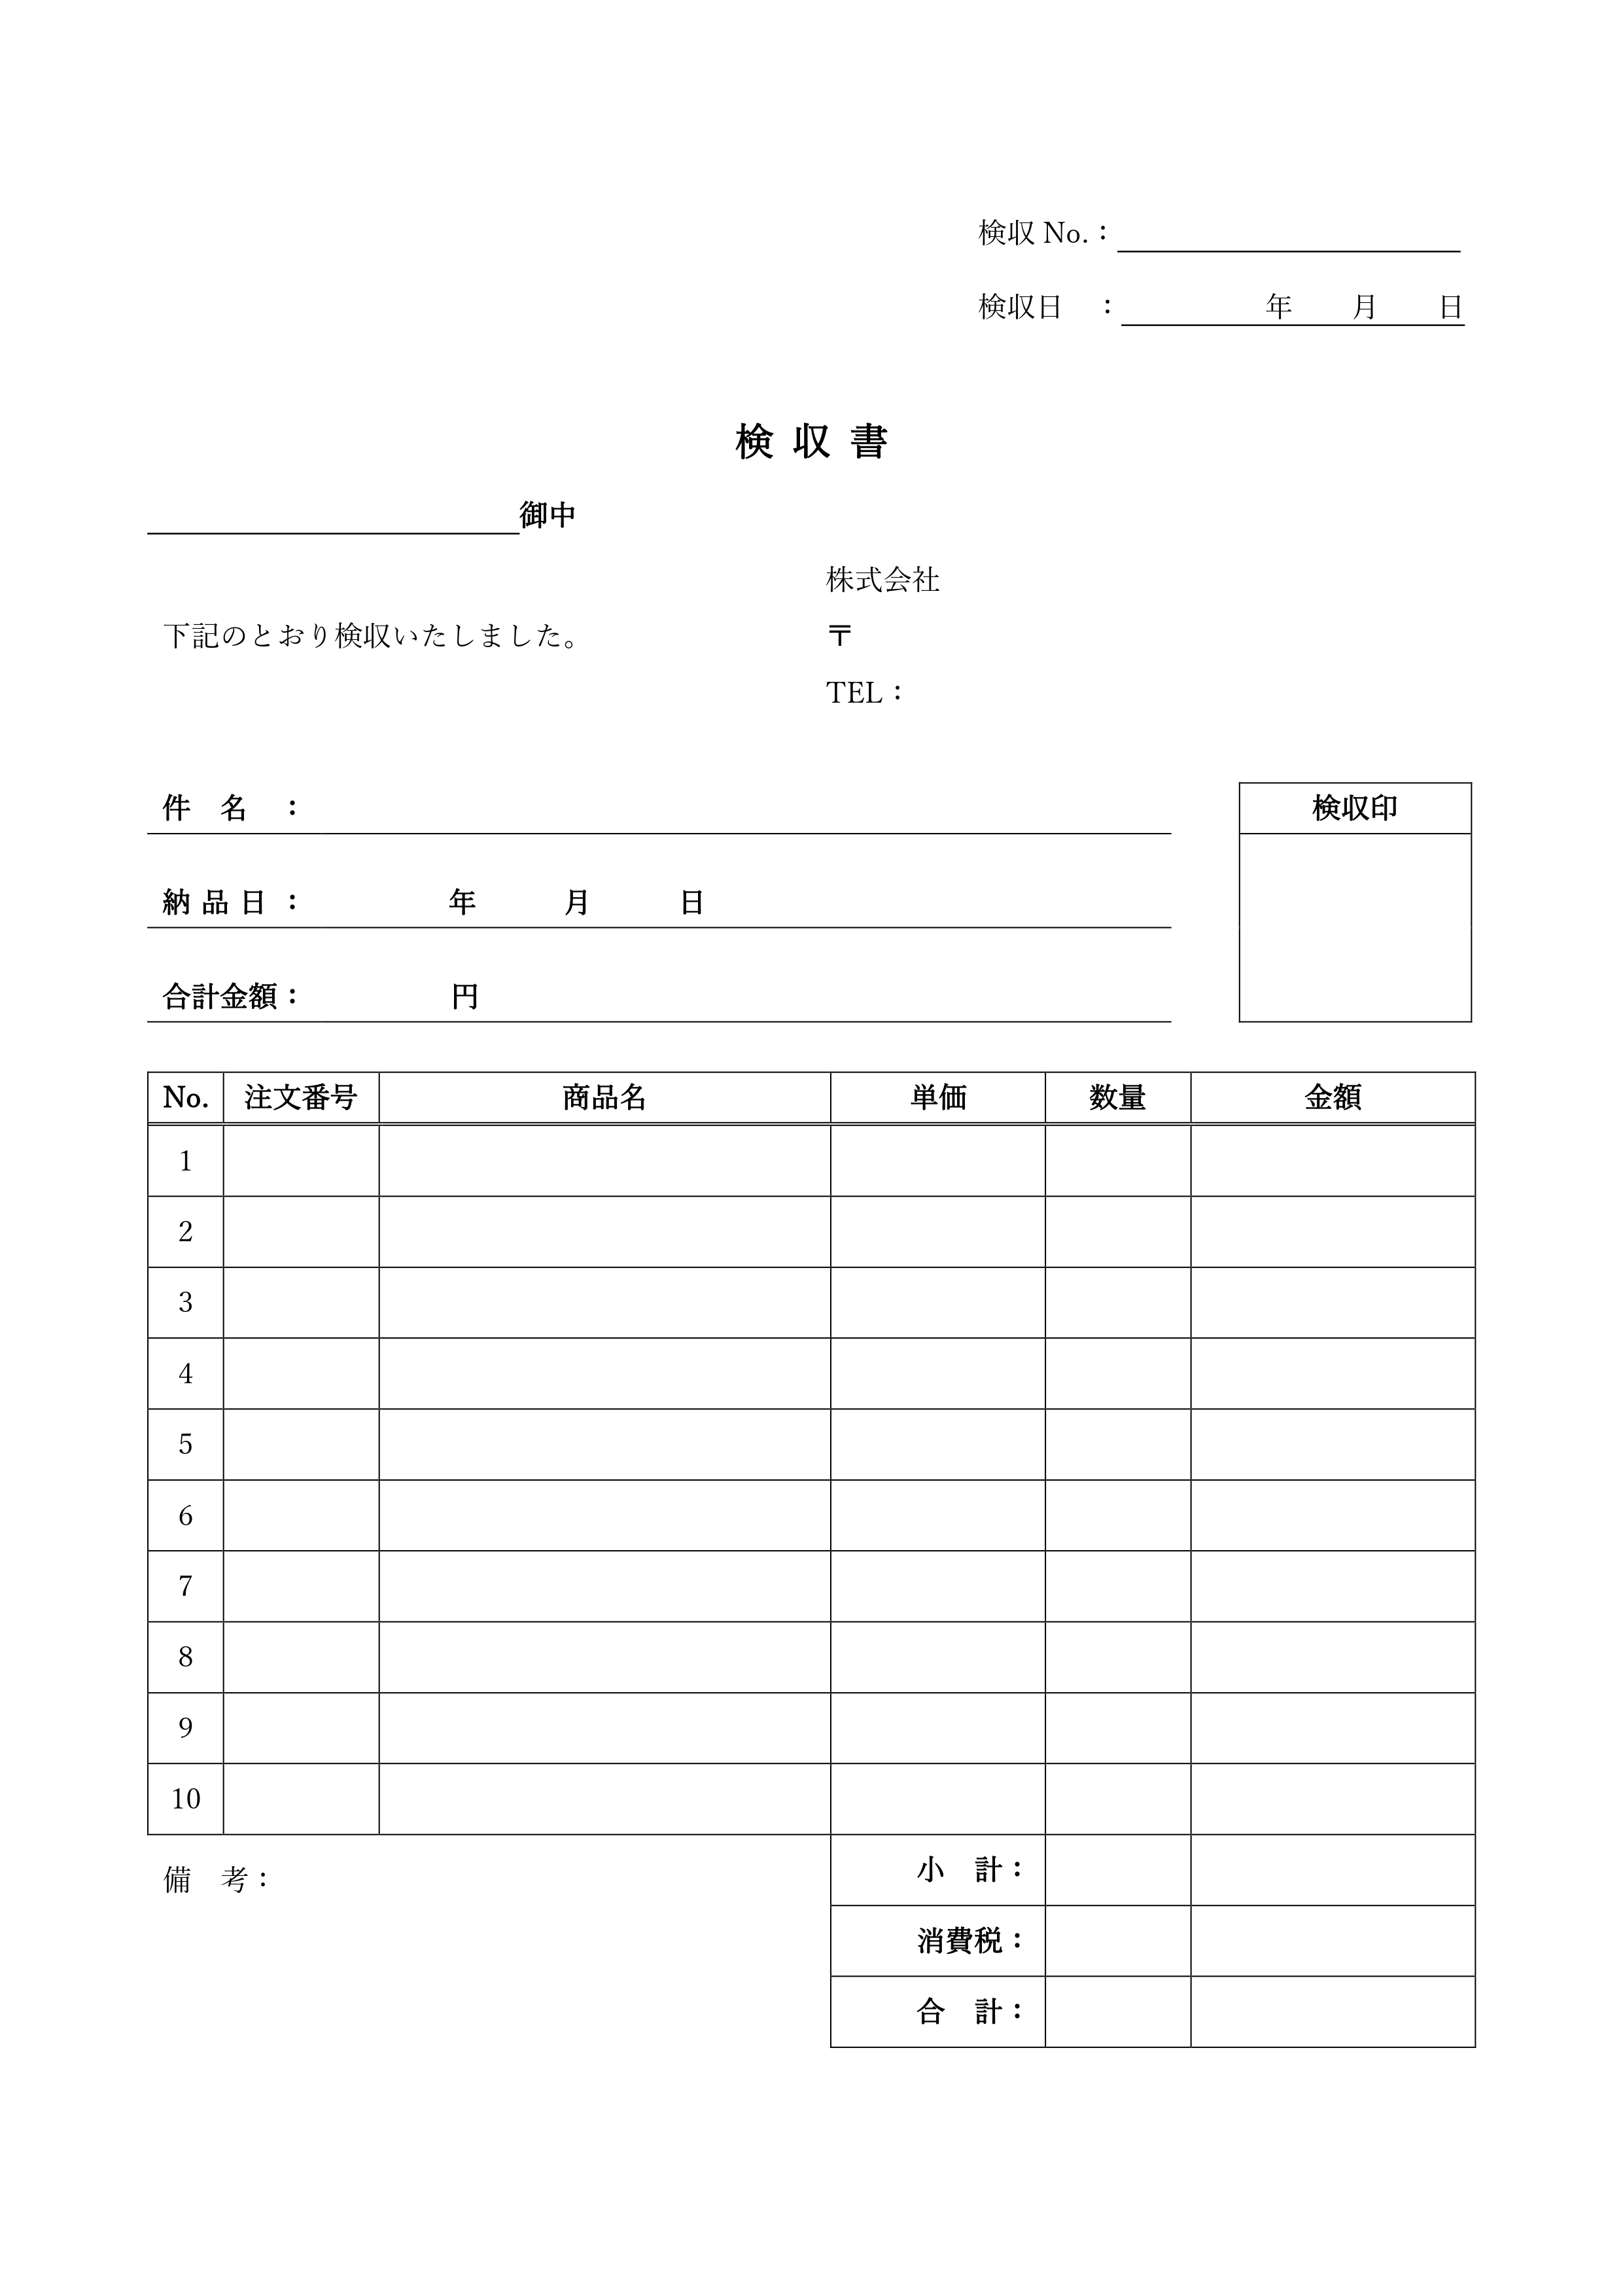
\includegraphics[width=15cm]{image/06-discussion/experiment_A.jpg}
            }
        \caption{実験対象である電子文書の帳票画像A}
        \label{fig:experiment_A}
    \end{center}
\end{figure}

\begin{figure}[t]
    \begin{center}
        \fbox{
            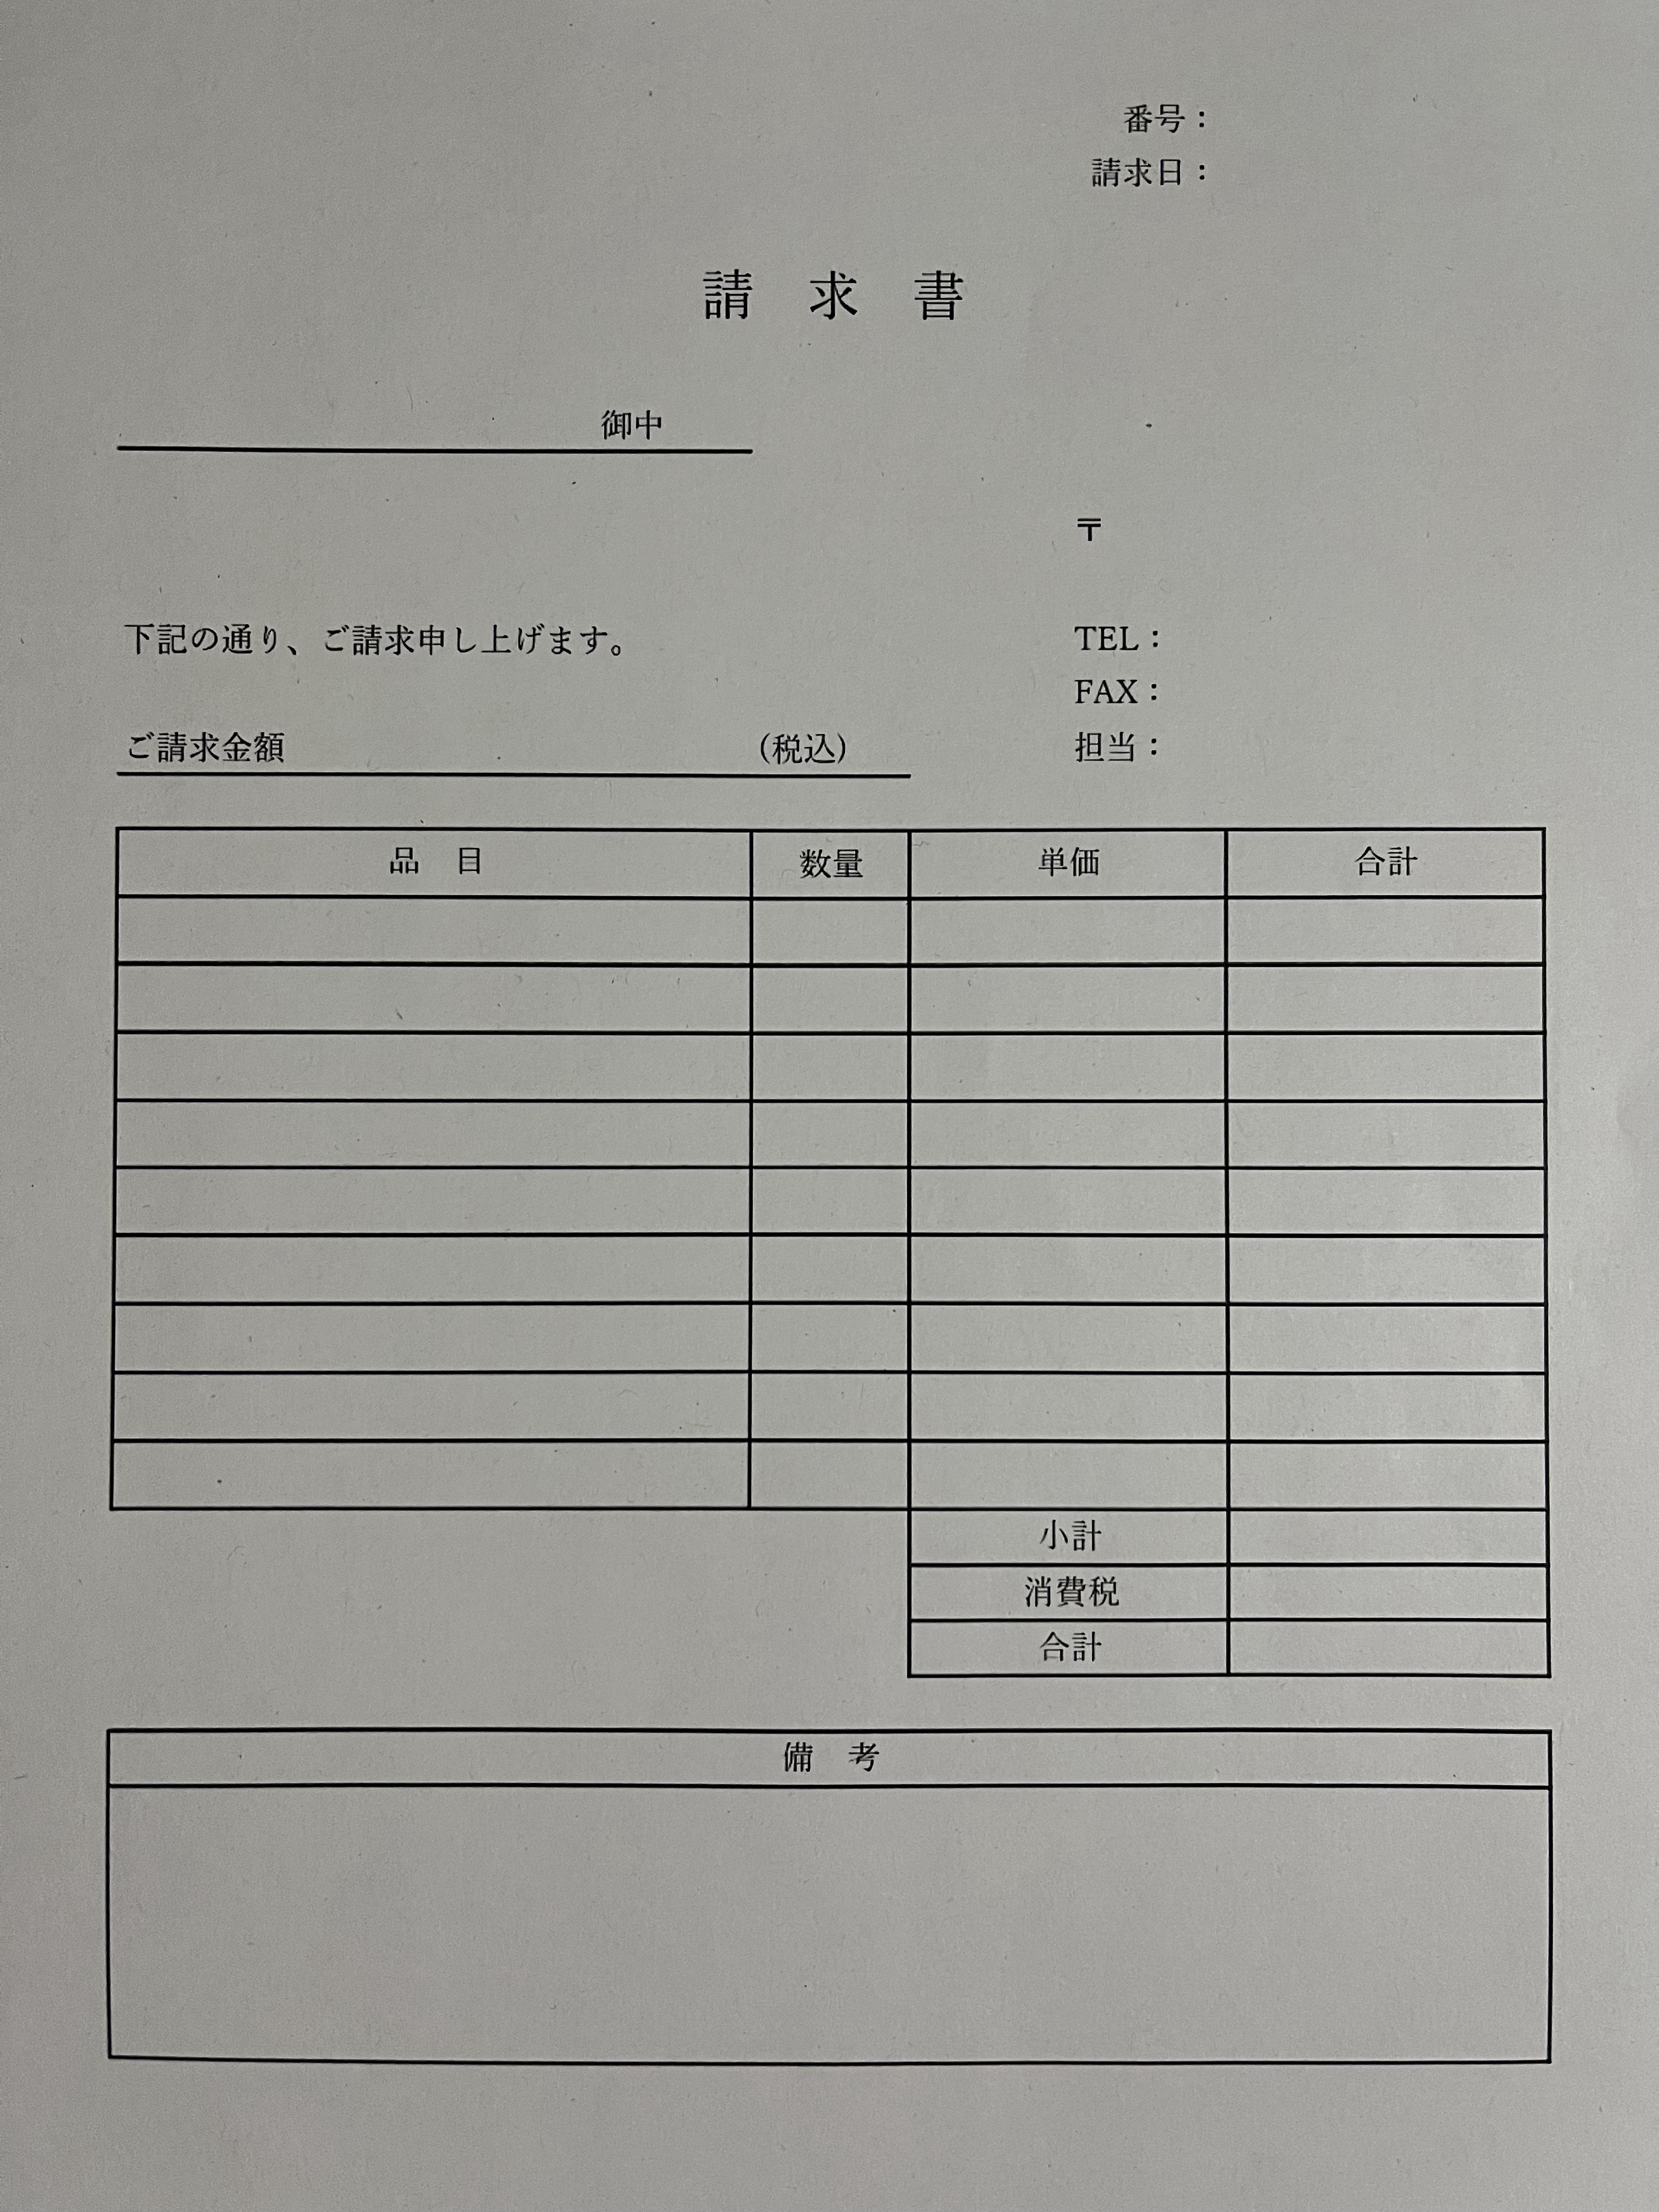
\includegraphics[width=15cm]{image/06-discussion/experiment_B.jpg}
        }
        \caption{実験対象である電子化文書の帳票画像B}
        \label{fig:experiment_B}
    \end{center}
\end{figure}

実験は、宮崎大学工学部情報システム工学科に所属する学部4年生2名、および修士1年生3名、2年生1名の計6名を対象として行った。

実験方法は、被験者6名をグループ$\alpha$とグループ$\beta$の2グループに分けて行う。
グループ$\alpha$は、図\ref{fig:experiment_A}の帳票画像Aに対して、試作したツールを適用せず、PhotolizeのGUIツールのみを用いて電子フォーム記入欄を配置してもらう。
次に、図\ref{fig:experiment_B}の帳票画像Bに対して、試作したツールを適用し、修正対象の電子フォーム記入欄を修正し、電子フォーム記入欄を配置してもらう。
グループ$\beta$は、図\ref{fig:experiment_A}の帳票画像Aに対して、試作したツールを適用し、修正対象の電子フォーム記入欄を修正し、電子フォーム記入欄を配置してもらう。
次に、図\ref{fig:experiment_B}の帳票画像Bに対して、試作したツールを適用せず、PhotolizeのGUIツールのみを用いて電子フォーム記入欄を配置してもらう。

被験者のグループ分けと実験手法を、表\ref{tb:experiment_case}に示す。

\begin{table}[t]
	\centering
	\caption{被験者のグループ分けと実験手法}
    \label{tb:experiment_case}
    \begin{tabular}{cc}
        \begin{minipage}[c]{0.5\hsize}
            \centering
            \begin{tabular}{c|c}
                グループ & 被験者 \\
                \hline \hline
                \multirow{3}{*}{グループ$\alpha$} & 被験者1 \\
                                               & 被験者2 \\
                                               & 被験者3 \\
                                        \hline
                \multirow{3}{*}{グループ$\beta$} & 被験者4 \\
                                              & 被験者5 \\
                                              & 被験者6
	        \end{tabular}
        \end{minipage} &
        \begin{minipage}[c]{0.5\hsize}
            \centering
            \begin{tabular}{c|c|c}
                グループ & 帳票画像 & 手法 \\
                \hline \hline
                \multirow{2}{*}{グループ$\alpha$} & 帳票画像A & GUIツールのみ \\
                                               & 帳票画像B & 試作ツール + 修正 \\
                                        \hline
                \multirow{2}{*}{グループ$\beta$} & 帳票画像A & 試作ツール + 修正 \\
                                              & 帳票画像B & GUIツールのみ
            \end{tabular}
        \end{minipage}
    \end{tabular}
\end{table}

なお、試作したツールで取得した領域座標、および、ラベルについては、間違っている可能性がある。
修正対象とする電子フォーム記入欄を、以下に示す。

\begin{itemize}
    \item 誤検出によって、帳票画像記入欄が存在しない場所に、電子フォーム記入欄を配置したもの。
    \item 帳票画像内に存在する帳票画像記入欄を検出できず、電子フォーム記入欄を配置できていないもの。
    \item 本来想定するラベルとは異なるラベルを割り付けたもの。
\end{itemize}

実験で計測する時間について、試作したツールを適用し、JSONファイルと2枚の領域強調画像を出力するまでの時間を、実行時間と呼ぶ。
また、電子フォーム記入欄の配置が完了するまでの時間を、配置時間と呼ぶ。

実験にあたり、PhotolizeのGUIツールを用いて、電子フォーム記入欄を配置する。
例えば、「個数」を記入する帳票画像記入欄には、「数値」の電子フォーム記入欄を選択し、ウインドウに表示する帳票画像内にドラッグすることで、電子フォーム記入欄を配置できる。
配置した電子フォーム記入欄については、矩形であり、各頂点と各辺の中点をドラッグすることで、拡縮を行う。
なお、Photolizeを利用するにあたり、記入する内容に適する種類の電子フォーム記入欄を選択して配置することで、ラベルを考慮したとみなす。
ラベルの種類については、試作したツールにおける日付(date)、文字列(string)、数値(number)に対応するよう、それぞれ日付/時刻、単一行テキスト、数値の3種類の電子フォーム記入欄のみを用いる。
試作したツールを適用し、PhotolizeのGUIツールで電子フォーム記入欄を配置した結果を修正する場合の実験手順を、以下に示す。

\begin{enumerate}
    \item 開始前に、実験対象の帳票画像とPhotolizeについて説明し、Photolizeにおける電子フォーム記入欄の配置操作も併せて説明する。
    \item 実行時間を計測する。
    \item PhotolizeのGUIツールを用いて、試作したツールが配置した電子フォーム記入欄を修正し、全ての電子フォーム記入欄を正しく配置するまでにかかる時間を計測する。
\end{enumerate}

試作したツールを適用せず、PhotolizeのGUIツールのみを用いて、電子フォーム記入欄を配置する場合の実験手順を、以下に示す。

\begin{enumerate}
    \item 開始前に、実験対象の帳票画像とPhotolizeについて説明し、Photolizeにおける電子フォーム記入欄の配置操作も併せて説明する。
    \item PhotolizeのGUIツールを用いて、全ての電子フォーム記入欄を正しく配置するまでにかかる時間を計測する。
\end{enumerate}

\subsection{電子フォーム記入欄を配置するまでにかかる時間に関する評価}\label{subsec:evalue_required_time}
本節では、電子フォーム記入欄を配置するまでにかかる時間について、評価を行う。

帳票画像A、Bについて、被験者6名の各計測時間とその合計時間を、表\ref{tb:result_time}に示す。
また、表\ref{tb:result_time}のうち、帳票画像Aにおける各計測時間の平均を、表\ref{tb:result_imageA_mean_time}に示す。
さらに、表\ref{tb:result_time}のうち、帳票画像Bにおける各計測時間の平均を、表\ref{tb:result_imageB_mean_time}に示す。
合計時間を算出する式を、式\ref{eq:sum_time}に示す。
なお、PhotolizeのGUIツールのみを用いて枠を配置した場合は、実行時間は0秒として計算する。

\begin{equation}\label{eq:sum_time}
    合計時間=実行時間+配置時間
\end{equation}

\begin{table}[t]
    \caption{被験者が電子フォーム記入欄を配置するまでにかかる時間(分:秒)}
	\label{tb:result_time}
    \centering
    \begin{tabular}{ccc||rrr} 
    グループ & 被験者 & 帳票画像 & 実行時間 & 配置時間 & 合計時間 \\
    \hline \hline
    
    \multirow{6}{*}{グループ$\alpha$} & \multirow{2}{*}{被験者1} & 帳票画像A & 00:00 & 08:49 & 08:49 \\ % 宮下さん M2  
                                                            & & 帳票画像B & 01:10 & 03:49 & 04:59 \\ 
                                                            
                                    & \multirow{2}{*}{被験者2} & 帳票画像A & 00:00 & 07:32 & 07:32 \\ % 田中くん B4
                                                            & & 帳票画像B & 01:12 & 03:18 & 04:30 \\
                                                            
                                    & \multirow{2}{*}{被験者3} & 帳票画像A & 00:00 & 10:03 & 10:03 \\ % 柿木さん M1
                                                            & & 帳票画像B & 01:30 & 02:50 & 04:20 \\
                                                            \hline
    \multirow{6}{*}{グループ$\beta$} & \multirow{2}{*}{被験者4} & 帳票画像A & 01:26 & 02:48 & 04:11 \\ % 高倉さん M1
                                                            & & 帳票画像B & 00:00 & 07:11 & 07:11 \\
                                                            
                                    & \multirow{2}{*}{被験者5} & 帳票画像A & 01:20 & 02:38 & 03:58 \\ % 翁長さん M1
                                                            & & 帳票画像B & 00:00 & 07:32 & 07:32 \\ 
                                                            
                                    & \multirow{2}{*}{被験者6} & 帳票画像A & 01:33 & 02:21 & 03:54 \\
                                                            & & 帳票画像B & 00:00 & 06:56 & 06:56 \\ 

    \end{tabular}
\end{table}

\begin{table}[t]
	\centering
    \begin{tabular}{cc}
        \begin{minipage}[c]{0.5\hsize}
            \centering
            \caption{帳票画像Aにおける各計測時間の平均(分:秒)}
            \label{tb:result_imageA_mean_time}
            \begin{tabular}{c|rrr}
                グループ & 実行時間 & 配置時間 & 合計時間 \\
                \hline \hline
                グループ$\alpha$ & 00:00 & 08:48 & 08:48 \\
                グループ$\beta$ & 01:26 & 02:36 & 04:02 \\
	        \end{tabular}
        \end{minipage} &
        \begin{minipage}[c]{0.5\hsize}
            \centering
            \caption{帳票画像Bにおける各計測時間の平均(分:秒)}
            \label{tb:result_imageB_mean_time}
            \begin{tabular}{c|rrr}
                グループ & 実行時間 & 配置時間 & 合計時間 \\
                \hline \hline
                グループ$\alpha$ & 01:12 & 03:19 & 04:31 \\
                グループ$\beta$ & 00:00 & 07:13 & 07:13 \\
            \end{tabular}
        \end{minipage}
    \end{tabular}
\end{table}

表\ref{tb:result_imageA_mean_time}より、帳票画像Aに関する合計時間は、グループ$\alpha$がグループ$\beta$よりも平均で4分46秒(約54.17\%)短い。
同様に、表\ref{tb:result_imageB_mean_time}より、帳票画像Bに関する合計時間は、グループ$\beta$がグループ$\alpha$よりも平均で2分42秒(約37.41\%)短い。
以上の結果から、試作したツールは、電子フォーム記入欄を配置する時間の削減について、有用であることがわかった。

% \begin{table}[t]
% 	\caption{ケース$\alpha$の被験者が配置完了までにかかる時間(分:秒)}
% 	\label{tb:result_caseA_time}
% 	\centering
% 	\begin{tabular}{cc||rrrr|r}
% 		被験者 & 帳票画像 & 実行時間 & 配置時間 & 合計時間 \\
%         \hline \hline

% 		% 宮下さん M2
% 		\multirow{2}{*}{被験者1} & 帳票画像A & 00:00 & 08:49 & 08:49 \\
% 		                        & 帳票画像B & 01:10 & 03:49 & 04:59 \\
%                                 \hline

% 		% 田中くん B4
% 		\multirow{2}{*}{被験者2} & 帳票画像A & 00:00 & 07:32 & 07:32 \\
%                                 & 帳票画像B & 01:12 & 03:18 & 04:30 \\
%                                 \hline

% 		% 柿木さん M1
% 		\multirow{2}{*}{被験者3} & 帳票画像A & 00:00 & 10:03 & 10:03 \\
%                                 & 帳票画像B & 01:30 & 2:50 & 04:20 \\
%                                 \hline \hline

% 		% 平均
% 		\multirow{2}{*}{平均}  & 帳票画像A & 00:00 & 08:48 & 08:48 \\
%                               & 帳票画像B & 01:12 & 03:19 & 04:31 \\
% 	\end{tabular}
% \end{table}

% \begin{table}[t]
% 	\caption{ケース$\beta$の被験者が配置完了までにかかる時間(分:秒)}
% 	\label{tb:result_caseB_time}
% 	\centering
% 	\begin{tabular}{rc||rrrr|r}
% 		被験者 & 帳票画像 & 実行時間 & 配置時間 & 合計時間 \\
%         \hline \hline

% 		% 高倉さん M1
% 		\multirow{2}{*}{被験者4} & 帳票画像A & 01:26 & 02:48 & 04:11 \\
%                                 & 帳票画像B & 00:00 & 07:11 & 07:11 \\
%                                 \hline

% 		% 翁長さん M1
% 		\multirow{2}{*}{被験者5} & 帳票画像A & 01:20 & 02:38 & 03:58 \\
%                                 & 帳票画像B & 00:00 & 07:32 & 07:32 \\
%                                 \hline

% 		%
% 		\multirow{2}{*}{被験者6} & 帳票画像A & &  &  \\
%                                 & 帳票画像B & 00:00 &  &  \\
%                                 \hline \hline

% 		% 平均
% 		\multirow{2}{*}{平均}   & 帳票画像A &  &  &  \\
%                                & 帳票画像B & 00:00 &  &  \\
% 	\end{tabular}
% \end{table}



\subsection{配置した電子フォーム記入欄の精度に関する評価}\label{subsec:evalue_accuracy}
本節では、配置した電子フォーム記入欄の精度について評価する。
なお、精度の評価は、領域座標とラベルについての、それぞれの適合率と再現率を算出することで行う。

それぞれの適合率、および、再現率を算出する式を、以下に示す。
なお、正しくラベルを割り付けた電子フォーム記入欄は、配置した電子フォーム記入欄の位置が正しいことを前提とする。

\begin{equation}
    領域座標の適合率=\frac{正しく配置した電子フォーム記入欄の数}{出力した領域座標の数}
\end{equation}

\begin{equation}
    領域座標の再現率=\frac{正しく配置した電子フォーム記入欄の数}{帳票画像記入欄の数}
\end{equation}

\begin{equation}
    ラベルの適合率=\frac{正しくラベルを割り付けた電子フォーム記入欄の数}{出力した領域座標の数}
\end{equation}

\begin{equation}
    ラベルの再現率=\frac{正しくラベルを割り付けた電子フォーム記入欄の数}{帳票画像記入欄の数}
\end{equation}

領域座標の適合率と再現率の平均を、表\ref{tb:result_rect_accuracy}に示す。
また、ラベルの適合率と再現率の平均を、以下の表\ref{tb:result_label_accuracy}に示す。

\begin{table}[t]
    \centering
    \begin{minipage}[h]{0.47\linewidth}
        \caption{出力した領域座標の適合率と再現率}
        \label{tb:result_rect_accuracy}
        \centering
        \begin{tabular}{r|c|c}
            帳票画像 & 適合率 & 再現率 \\
            \hline \hline
            帳票画像A & 0.806 & 1.000 \\
            帳票画像B & 0.857 & 0.875 \\
        \end{tabular}
    \end{minipage}
    \begin{minipage}[h]{0.47\linewidth}
        \caption{出力したラベルの適合率と再現率}
        \label{tb:result_label_accuracy}
        \centering
        \begin{tabular}{r|c|c}
            帳票画像 & 適合率 & 再現率 \\
            \hline \hline
            帳票画像A & 0.731 & 0.907 \\
            帳票画像B & 0.674 & 0.688 \\
        \end{tabular}
    \end{minipage}
\end{table}

表\ref{tb:result_rect_accuracy}、および表\ref{tb:result_label_accuracy}より、2枚の帳票画像に共通して、領域座標およびラベルの再現率は、適合率に比べ高いことがわかる。
この結果より、試作したツールを用いて修正する場合は、電子フォーム記入欄を配置する修正の回数よりも、不要に配置した電子フォーム記入欄を削除する修正の回数が多いと推測できる。
電子フォーム記入欄を配置する場合は、ラベルを考慮しつつ、位置を調整する必要がある。
一方、電子フォーム記入欄を削除する場合は、その必要がないため、電子フォーム記入欄を配置する場合と比較して、手間がかからない。
よって、試作したツールは、電子フォーム記入欄を配置する手間の削減について、有用であることがわかった。

しかし、表\ref{tb:result_rect_accuracy}、および表\ref{tb:result_label_accuracy}より、領域座標とラベルについて、領域座標の適合率を除き、帳票画像Bにおける適合率と再現率は、帳票画像Aにおける適合率と再現率と比較して低い。
これについては、帳票画像Bに、矩形および下線部で示されていない記入欄を含むことと、帳票画像Bを撮影した環境によって、二値化の結果に影響があり、一部の領域を検知できなかったことが原因である。
これらの問題については、\ref{sec:problems}節で後述する。

% \begin{equation}
%     ラベルの適合率=\frac{正しくラベルを割り付けた電子フォーム記入欄の数}{出力した領域座標の数}
% \end{equation}

% \begin{equation}
%     ラベルの再現率=\frac{正しくラベルを割り付けた電子フォーム記入欄の数}{帳票画像記入欄の数}
% \end{equation}



% 領域座標について、精度に関する評価指標をまとめた表を、表\label{tb:result_accuracy}に示す。

% \begin{table}[t]
% 	\caption{本ツールが出力した領域座標の精度に関する評価指標}
% 	\label{tb:result_accuracy}
% 	\centering
% 	\begin{tabular}{cc||rrrr|r}
% 		帳票画像 & 配置する電子フォーム記入欄の数 & 適合率 & 再現率 & 正解率 \\
%         \hline \hline
%         帳票画像A & 54 & 00:00 & 08:49 & 08:49 \\
%         帳票画像B & 48 & 01:10 & 03:49 & 04:59 \\
%         \hline
% 	\end{tabular}
% \end{table}

% \begin{table}[t]
% 	\caption{ケース$\alpha$の被験者が正しく配置した電子フォーム記入欄}
% 	\label{tb:result_accuracy}
% 	\centering
% 	\begin{tabular}{cc||rrrr|r}
% 	     & 再現率 & 適合率 & 正解率 & 合計時間 \\
%         \hline \hline

% 		% 宮下さん M2
% 		\multirow{2}{*}{被験者A} & 帳票画像A & 00:00 & 08:49 & 08:49 \\
% 		                        & 帳票画像B & 01:10 & 03:49 & 04:59 \\
%                                 \hline

% 		% 
% 		\multirow{2}{*}{被験者B} & 帳票画像A & 00:00 &  &  \\
%                                 & 帳票画像B &  &  &  \\
%                                 \hline

% 		%
% 		\multirow{2}{*}{被験者C} & 帳票画像A & 00:00 & 00:19 &  \\
%                                 & 帳票画像B & 00:57 &  &  \\
%                                 \hline

% 		%
% 		\multirow{2}{*}{被験者D} & 帳票画像A & 00:00 & 00:19 &  \\
%                                 & 帳票画像B & 00:57 &  &  \\
%                                 \hline \hline

% 		% 平均
% 		\multirow{2}{*}{平均}  & 帳票画像A & 00:00 &  &  \\
%                               & 帳票画像B &  &  &  \\
% 	\end{tabular}
% \end{table}




\section{関連ツール}\label{sec:relation_tools}
本節では、本研究で試作した記入欄の検出およびラベル付与手法と、関連ツールを比較する。
電子フォーム作成ツールに、株式会社シムトップスのi-Reporter\cite{i-Reporter}や、インフォテック株式会社のCreate!Form\cite{Create!Form}がある。
これらの電子フォーム作成ツールを用いることによって、帳票をデザインしたExcelファイルと、画像ファイルを入力として、電子フォームを作成することができる。
帳票をデザインしたExcelファイルを入力とすることにより、記入欄の位置をセル単位で取得することができ、セルに設定した書式設定を保持した状態で、電子フォームを自動で作成できる。
しかし、紙媒体のレイアウトをもとにExcelファイルで構成を書き直す必要があり、レイアウトが変わる場合がある。
また、帳票の画像ファイルを入力とした場合は、入力する帳票画像を背景とするため、レイアウトは変わらない。
しかし、GUIツールを用いたマウス操作で記入欄を配置する必要があるため、電子フォームの作成に手間と時間がかかる。
また、サイボウズ社が提供するクラウドサービスであるkintone\cite{kintone}を利用し、データベースに保存したデータから、記入済みの帳票を自動作成する外部連携サービスに、トヨクモ株式会社のPrintCreator\cite{PrintCreator}や、オーサムジョブ合同会社のk-Report\cite{k-Report}がある。
しかし、背景となるPDFファイルを用意し、電子フォーム記入欄をGUIツールのマウス操作で配置することによって、帳票のテンプレートを作成する必要があり、手間と時間がかかる。
このように、既存の電子フォーム作成ツールやサービスは、帳票のレイアウトを変更しないことと、電子フォームの作成にかかる手間と時間を削減することを両立できない。

試作したツールは、レイアウトを変更せず、帳票画像記入欄を自動検出し、バリデーションチェックに必要である記入内容のデータ型をラベルとして割り付け、JSONファイルとして出力できる。
また、JSONファイルの内容を人間が確認しやすくするため、検出した帳票画像記入欄と、そのラベルを強調表示して、画像として出力できる。
これにより、レイアウトを変更せず、電子フォーム作成の時間と手間を削減できる。

\section{試作したツールの問題点}\label{sec:problems}
試作したツールの問題点を、以下に示す。

\begin{itemize}
    \item 記入内容を示す欄を、帳票画像記入欄として検出する\\
        矩形領域と下線部領域は、それぞれ矩形と直線を検出し、領域座標を取得したものである。
        領域座標取得部(\ref{sec:area_coords_obtainment_part}節を参照)において、文字情報を参照しないため、領域座標が記入する内容を示す欄か、帳票画像記入欄かを判別することができない。
        特に、矩形が隣接する形式の帳票である際、行または列が記入する内容を示す場合がある。
        これによって、記入する内容を示す欄の数だけ、不要に領域座標を出力してしまう。
        この問題点については、取得した領域座標と文字位置を参照し、領域座標の中心点から一定の範囲内であれば、出力から除外することで解決できると考える。
    \item 割り付けるラベルが不安定である\\
        試作したツールにおいて、割り付けるラベルは、文字情報とYouriの出力に依存する。
        Tesseract-OCRは、100\%正確に画像から文字を認識することができず、本来認識するべき文字とは別の文字として認識する場合がある。
        例えば、「は」と「ば」などの、視覚的な違いが少ない文字や、「品」と「口」などの、一部に別の漢字を含む漢字が存在する場合は、誤認識する可能性が高い。
        この誤認識によって、\ref{sec:result_rect}節で述べたような、誤ったラベルを割り付ける場合がある。
        また、Youriの出力は、誤って属性を推測する場合があり、かつ出力が常に一定ではない。
        Tesseract-OCRとYouriの2つの不安定な出力によって決定するため、割り付けるラベルが不安定である。
        この問題点については、他の光学文字認識ソフトウェアの利用や、プロンプトの改善によって解決できると考える。
    \item 特殊なレイアウトの帳票画像については、精度が低下する\\
        欄の一部に色が付いているもの、絵や押印を含むものなど、記入欄と文字以外のものが帳票画像にある場合は、領域座標を取得する精度と、ラベルを付与する精度の両方が低下する。
        これは、二値化の結果に影響を及ぼすためである。
        特に、青や紫などの暗色は、グレースケール画像において画素値が高くなり、二値化した際に黒となる可能性が高い。
        二値化によって、記入欄と文字以外に黒の画素が存在する場合、誤検出の可能性が高くなる。
        この問題点については、二値化手法の変更や、一定範囲内に閾値を超える数の黒の画素を認識した場合は、隣接する黒の画素を白に変換することで解決できると考える。
    \item 記入内容を示す文字が右にある場合は、他の文字の属性をラベルとして割り付けてしまう\\
        \ref{subsec:label_link_processing}節で述べたラベルを割り付ける手法は、記入内容を示す文字が左にある場合のみに正常に動作する。
        記入内容を示す文字が右にある場合もラベルの更新を行った場合、行ごとに共通したラベルを割り付けてしまうため、1列ごとに記入内容を決定する形式の帳票に対しては、正常にラベルを割り付けることができない。
        この問題点については、帳票の記入方向を検知し、検知した結果によってラベルを更新する順番を変更することで解決できると考える。
    \item 記入欄の一部が、矩形または下線部で表示されていない場合は、領域座標を取得できない\\
        帳票画像記入欄は、矩形または下線部で示されていることを前提とするため、文字のみで帳票画像記入欄を示すものについては、領域座標を取得できない。
        この問題点については、文字認識の結果、品詞が名詞である単語のみを認識した場合は、その単語のバウンディングボックスと同じ矩形を右に配置することで解決できると考える。
    \item 撮影環境によって、矩形と下線部の検出、および文字認識の精度が低下する\\
        図\ref{fig:experiment_B}のような電子化文書の画像を入力とした場合は、電子文書の画像と比較して、矩形と下線部の検出、および文字認識の精度が低い傾向にある。
        これは、DeblurGANv2で除去できなかったブレや、撮影場所の明るさ、撮影時に影が映ることなどの、撮影環境が二値化の結果に影響を及ぼすためである。
        この問題点については、陰影除去などの別の画像処理を加えることで解決できると考える。
\end{itemize}